%mci-term-paper.tex 
\documentclass[12pt]{article}
\usepackage{times}
\usepackage{amsmath,amssymb,latexsym}
\usepackage[round,sort]{natbib}
\usepackage{multirow,array}
\usepackage{fancyhdr}
\usepackage{lastpage}
\usepackage{graphicx}
\usepackage[bottom]{footmisc}
\graphicspath{ {mci-term-paper-images/} }
\usepackage[T1]{fontenc}
\usepackage{mathptmx}
\usepackage{tabu}
\usepackage{textcomp}
\usepackage{stata}
\usepackage{listings}
\usepackage[a4paper,margin=1.0in]{geometry}
\usepackage{multirow}
\usepackage{caption}
\usepackage{setspace}
\usepackage{verbatim}
\usepackage{pdflscape}
\usepackage{longtable}
\usepackage{hyperref}
\setlength{\parindent}{4pt}
\setlength{\parskip}{1.3em}
\hypersetup{
    colorlinks=true,
    linkcolor=blue,
    filecolor=magenta,      
    urlcolor=cyan,
    citecolor=magenta,
}
\lstset{
basicstyle=\ttfamily,
columns=flexible,
breaklines=true
}
\newenvironment{hypothesis}{
  	\itshape
  	\leftskip=\parindent \rightskip=\parindent
  	\noindent\ignorespaces}
	
\setlength\parindent{0pt}
\pagestyle{fancy}
\fancyhf{}
\lhead{Does inventor mobility affect productivity?}
\rfoot{Page \thepage  \ of \pageref{LastPage}}
\rhead{Iyenggar}
\newcommand\question[2]{\vspace{1em}\hrule\vspace{1em}\textbf{#1}{ #2}\vspace{1em}\hrule\vspace{1em}}

\begin{document}
\title{\LARGE Does inventor mobility affect productivity?\\ \Large \textit{Methods for Causal Inference} course term paper}
\author{Ashwin Iyenggar  (1521001) \\ ashwin.iyenggar15@iimb.ernet.in} 
\large

\maketitle
\thispagestyle{empty}

\begin{abstract}
\large \noindent Using patent inventions data, I attempt to investigate if inventor mobility influences the productivity of those inventors. I leverage a database of worldwide urban regions  obtained from remote sensing to demonstrate a significant positive correlation between both inter-region mobility  and inter-country mobility and future invention productivity of inventors. I discuss two additional approaches to investigate if a causal explanation exists for this relationship but leave empirical analysis for future work. While the empirical results are incomplete, the current work extends prior work on mobility of inventors by attempting to quantify the direct effects of  mobility on inventor productivity.
\end{abstract}
{Keywords:} Inventor productivity, Inventor mobility, Economic geography
\onehalfspacing
\section{Introduction}
Scholars have suggested that inventors carry knowledge with them when they move \citep{Almeida1999}. While the literature on knowledge flows has investigated the localized nature of knowledge flow driven by the inter-firm mobility of inventors \citep{Jaffe1993, Almeida1999, Alcacer2006a}, we understand very little about the effects of broad mobility of inventors on future inventive productivity. Since firms, regions and countries seek to organize themselves so as to attract the best inventors so as to produce the highest level of innovative output, an understanding of the mobility effects of inventive productivity becomes an important aspect innovation policy. In this paper I ask if  the variation in inventor mobility can explain the variation in invention productivity?

Agglomeration economies have been suggested as one reason for localized movement of inventors. These agglomeration economies arise due to labor pooling advantages, economies of specialization of local suppliers, and knowledge spillovers \citep{Porter1990, Krugman1991}. However regions vary in their inventive output \citep{Agrawal2014} and the nature of knowledge flows in a region may be one source of this variation within regions. In this study therefore, I propose to expand the context to not just localized agglomerations but to all movements of inventors. By doing so, I expect to understand if there is a clear impact of mobility itself on invention productivity. In other words, what is the relationship between the movement of some inventors into or out of a region and the average productivity of inventions from those inventors?\par

There has been a long and illustrious scholarly tradition highlighting the agglomeration characteristics of economic regions, going back at least as far as \cite{Marshall1890}, whose original work was published in 1890. More recently, scholars over the last three decades have demonstrated the paper trail of these knowledge spillovers through the study of patent citations (e.g., \cite{Jaffe1993, Almeida1999}). This tradition of scholarship has further shaped our theoretical understanding of knowledge spillovers through mechanisms such as the effects of inventor mobility (e.g., \cite{Almeida1999}), differential Intellectual Property Rights environments across locations (e.g., \cite{Zhao2006}) and of the role of international geography (e.g., \cite{Singh2007}).  The nature and extent of the geographical mobility of inventors  observed  in practice is highly heterogenous across locations, firms and legal environments. This raises the opportunity to study if  a causal effect exists between mobility of inventors and their future productivity. The question is assumes greater significance in the environment surrounding the second machine age \citep{Mcafee2014} where inventors are expected to influence innovation outcomes in higher proportion. 

The innovation policy of emerging countries is influenced with the expectation that the presence of multinational R\&D will create value adding spillover effects. Productivity of inventors may  provide a richer proxy for value adding innovation. A better understanding of the effects of inventor mobility may therefore help to inform innovation policy. Additionally, work on this line may help to inform managerial decisions about how to organize R\&D teams around the world. Current theory seems to suggest both a positive effect due to knowledge spillovers \citep{Almeida1999} as well as a negative effect due to variation in IPR enforcement ability \citep{Zhao2006}. I therefore propose  the current empirical study to help determine an  answer to this question that is not completely explained by theory.

The rest of the paper is organized as follows. The next section explores the motivation of the current study. Hypotheses based on extant literature are then presented. I then describe the data and methods. The preliminary results are then presented, followed by a discussion of the results. I conclude with next steps and open questions for further research.

\section{Motivation}
I motivate this study by demonstrating two broad patterns.  First, as Figure ~\ref{fig:countrymoves} suggests,  there has been increased mobility of inventors across countries over the years. Not only is the incidence of across-country mobility higher, but there is heterogeneity in the extent across countries and regions. Figure ~\ref{fig:regionmoves} furthers this aspect by depicting the trend in across-region mobility of inventors. Second, Table ~\ref{sumstat} suggests that about 6\% of inventors moved  and only about 2\% of inventors moved country. 

\begin{figure}[h]
\begin{centering}
  \includegraphics[width=0.7\textwidth]{countrymoves}
  \caption{Country moves by year}
   \label{fig:countrymoves}
\end{centering}
\end{figure}

The two broad patterns together provide us both the motivation as well as the variation in the data to be able ask the question of whether the mobility of inventors affects invention productivity. It must be noted at this point that while we have data on inventors who moved and patented in their new location, and data on inventors who did not move and continued to patent at their existing location, the patents data itself does not provide us data on those inventors who moved but did not patent, and those who did not move and did not patent. This may cause us to either overestimate the effect of mobility or underestimate the effect of not moving. 

\begin{figure}[h]
\begin{centering}
  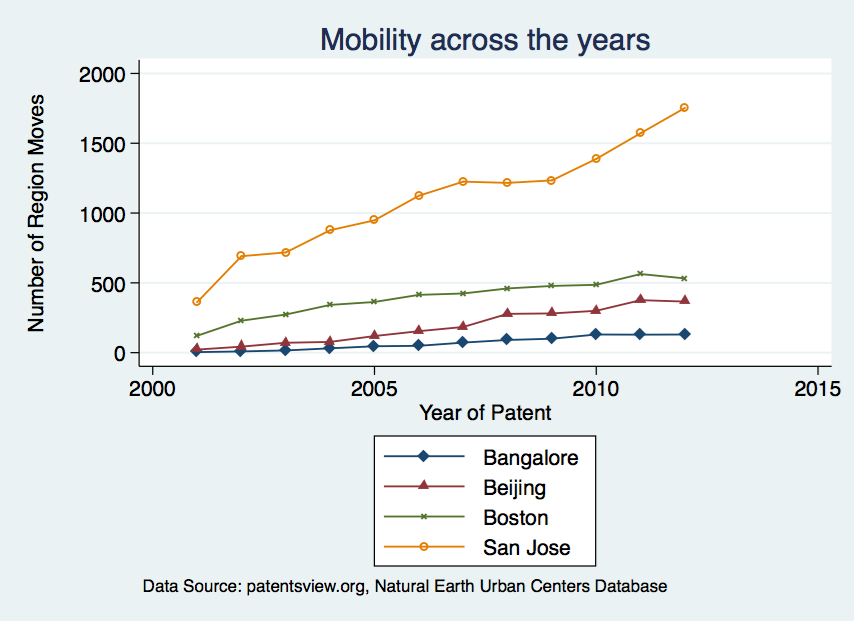
\includegraphics[width=0.7\textwidth]{regionmoves}
  \caption{Region moves by year}
   \label{fig:regionmoves}
\end{centering}
\end{figure}


\begin{table}[htbp]\centering \caption{Summary statistics \label{sumstat}}
\begin{tabular}{l c c  c}\hline\hline
\multicolumn{1}{c}{\textbf{Variable}} & \textbf{Mean}
 & \textbf{Std. Dev.} & \textbf{N}\\ \hline
Moved Region (MR) & 0.06 & 0.238  & 4368062\\
Moved Country (MC) & 0.021 & 0.143  & 4368062\\
Productivity & 1.79 & 2.647  & 4368062\\
Prior Patents of Inventor (PPI) & 4.716 & 16.718  & 4368062\\
Prior Patents of Team (PPT) & 24.557 & 112.7  & 3721064\\
\hline
\end{tabular}
\end{table}




\section{Theory}
In this section, I develop three hypothesis building off of prior literature on inventor mobility and knowledge spillovers. 

The literature on agglomeration economies and knowledge spillovers suggest that when inventors move across regions, that newer combinations of knowledge now become possible \cite{Jaffe1993, Almeida1999}. Literature would therefore predict better and more numerous inventions arising out of the movement of inventors. I therefore propose hypothesis 1 as follows:\par
\begin{hypothesis}{\\Hypothesis 1: An increase in the average mobility of inventors in a region increases the average productivity of  the inventor}\end{hypothesis}

\cite{Singh2007} suggests that inventors who were highly productive previously are likely to carry that after the move. I therefore propose hypothesis 2 as follows:\par
\begin{hypothesis}{\\Hypothesis 2: The effect in Hypothesis 1 is moderated positively by the strength of the prior pool of inventions by the inventor}\end{hypothesis}

Finally, the literature of weak and strong IPR suggests that teams within weak IPR locations are likely to integrate their knowledge within global organizations, thus leading to a lower standalone inventive output. I therefore propose hypothesis 3 as follows:\par
\begin{hypothesis}{\\Hypothesis 3: The effect in Hypothesis 1 is moderated negatively by the strength of the prior pool of inventions by the inventing team}\end{hypothesis}


\section{Data and Measures}

I derive all patents data for this study from patentsview.org. The dataset considered is for all USPTO patents filed in the period 1976 to 2015. For country definitions, I use the resources provided by \href{http://thematicmapping.org/downloads/world_borders.php}{Thematic Mapping}. To map location data of inventors to regions, I use urban centers data for worldwide locations from \href{http://www.naturalearthdata.com/downloads/10m-cultural-vectors/}{Natural Earth Data} that uses remote sensing data to determine urban agglomerations (a process developed in \cite{Schneider2003}).  While it has been common practice to use Metropolitan Statistical Areas (MSA) for analyses related to economic geography in the U.S., an equivalent measure is unavailable for the rest of the world. For comparability and consistency, I choose to use the urban centers definitions from \href{http://www.naturalearthdata.com/downloads/10m-cultural-vectors/}{Natural Earth Data} for all regions both within U.S. and outside U.S. Sample region definitions are depicted in Figure ~\ref{fig:SanJose} and ~\ref{fig:Bangalore} in the appendix. 

\subsection{Unit of Analysis}
The unit of analysis for this study is the \verb|inventor| - \verb|year|. For each inventor-year, I capture if the inventor moved in that year. As was previously discussed, the nature of our data is that we do not have data for years in which inventors did not patent. However for the years for which patents were applied for, we identify if there was a movement or not.

\subsection{Dependent Variable}
My primary dependent variable is the productivity of an inventor in a year.  I measure \texttt{productivity} by the number of patents invented by the inventor in the year and in two years succeeding that year. The dependent variable may be zero, or 1 or a value higher depending on the inventive productivity of the inventor.

\subsection{Explanatory Variables}
I use two primary explanatory variables - \texttt{between-region} mobility, and \texttt{between-country} mobility.  For each inventor-year,  I  determine mobility for the inventor in that year by comparing the region  of the previous patent to that of the current patent. If the region has not changed, I mark between-region mobility to zero for that inventor-year. Else \texttt{between-region} mobility is marked as one for that inventor-year.\par

Similarly, to determine \texttt{between-country} mobility for an inventor-year,  I  compare the country  of the previous patent to that of the current patent. If the country has not changed, I mark \texttt{between-country} mobility to zero for that inventor-year. Else \texttt{between-country} mobility is marked as one for that inventor-year.\par

I define two additional explanatory variables. \par
\texttt{Prior patents of inventor} (PPI) is intended to capture the inventor specific aspects and is computed by adding up the number of patents granted to the invented up to but not including the patents granted in the current year. \texttt{Prior patents of team} (PPT) is intended to capture the team specific aspects affecting inventor productivity. It is computed by summing up the number of patents granted to the most prolific of the inventors within the team (not including the focal inventor).

\subsection{Control Variables and Fixed Effects}
I use the technology classification defined by  \cite{Hall2001} to control for various technology subcategories. All models also include  year dummies so as to account for any year specific effects. Depending on the model run, we cluster standard errors at the region level, the country level or the technology subclass level.

\section{Results}
\begin{table}
\caption{Regression Results}
\begin{center}
\begin{tabular}{lccc}
\multicolumn{4}{c}{\begin{large}Regional Mobility of Inventors and Productivity of Inventors\end{large}} \\ \hline
 & (1) & (2) & (3) \\
VARIABLES & Productivity & Productivity & Productivity \\ \hline
\vspace{4pt} & \begin{footnotesize}\end{footnotesize} & \begin{footnotesize}\end{footnotesize} & \begin{footnotesize}\end{footnotesize} \\
Moved Region (MR) & 1.3974*** & 0.7966*** & 0.5571*** \\
\vspace{4pt} & \begin{footnotesize}(0.0997)\end{footnotesize} & \begin{footnotesize}(0.0531)\end{footnotesize} & \begin{footnotesize}(0.0556)\end{footnotesize} \\
Prior Patents of Inventor (PPI) &  & 0.0852*** & 0.0741*** \\
\vspace{4pt} & \begin{footnotesize}\end{footnotesize} & \begin{footnotesize}(0.0041)\end{footnotesize} & \begin{footnotesize}(0.0027)\end{footnotesize} \\
Prior Patents of Team (PPT) &  & 0.0004*** & 0.0005*** \\
\vspace{4pt} & \begin{footnotesize}\end{footnotesize} & \begin{footnotesize}(0.0001)\end{footnotesize} & \begin{footnotesize}(0.0001)\end{footnotesize} \\
MR x PPI &  &  & 0.0282*** \\
\vspace{4pt} & \begin{footnotesize}\end{footnotesize} & \begin{footnotesize}\end{footnotesize} & \begin{footnotesize}(0.0054)\end{footnotesize} \\
MR x PPT &  &  & -0.0005*** \\
\vspace{4pt} & \begin{footnotesize}\end{footnotesize} & \begin{footnotesize}\end{footnotesize} & \begin{footnotesize}(0.0002)\end{footnotesize} \\
Constant & 1.7123*** & 1.7258*** & 1.7404*** \\
 & \begin{footnotesize}(0.0894)\end{footnotesize} & \begin{footnotesize}(0.0468)\end{footnotesize} & \begin{footnotesize}(0.0504)\end{footnotesize} \\
\vspace{4pt} & \begin{footnotesize}\end{footnotesize} & \begin{footnotesize}\end{footnotesize} & \begin{footnotesize}\end{footnotesize} \\
Observations & 2,886,438 & 2,507,963 & 2,507,963 \\
$R^2$ & 0.0282 & 0.2940 & 0.3010 \\
Year FE & Yes & Yes & Yes \\
Technology FE & Yes & Yes & Yes \\
 Clustered SE & Region & Region & Region \\ \hline
\multicolumn{4}{c}{\begin{footnotesize} Robust standard errors in parentheses\end{footnotesize}} \\
\multicolumn{4}{c}{\begin{footnotesize} *** p$<$0.01, ** p$<$0.05, * p$<$0.1\end{footnotesize}} \\
\end{tabular}
\end{center}

\label{RR}
\end{table}

\begin{table}
\caption{Regression Results}
\begin{center}
\begin{tabular}{lccc}
\multicolumn{4}{c}{\begin{large}Regional Mobility of Inventors and Productivity of Inventors\end{large}} \\ \hline
 & (1) & (2) & (3) \\
VARIABLES & Productivity & Productivity & Productivity \\ \hline
\vspace{4pt} & \begin{footnotesize}\end{footnotesize} & \begin{footnotesize}\end{footnotesize} & \begin{footnotesize}\end{footnotesize} \\
Moved Region (MR) & 1.5681*** & 0.9204*** & 0.6239*** \\
\vspace{4pt} & \begin{footnotesize}(0.0926)\end{footnotesize} & \begin{footnotesize}(0.0606)\end{footnotesize} & \begin{footnotesize}(0.0654)\end{footnotesize} \\
Prior Patents of Inventor (PPI) &  & 0.0803*** & 0.0683*** \\
\vspace{4pt} & \begin{footnotesize}\end{footnotesize} & \begin{footnotesize}(0.0138)\end{footnotesize} & \begin{footnotesize}(0.0124)\end{footnotesize} \\
Prior Patents of Team (PPT) &  & 0.0003*** & 0.0005*** \\
\vspace{4pt} & \begin{footnotesize}\end{footnotesize} & \begin{footnotesize}(0.0000)\end{footnotesize} & \begin{footnotesize}(0.0000)\end{footnotesize} \\
MR x PPI &  &  & 0.0319*** \\
\vspace{4pt} & \begin{footnotesize}\end{footnotesize} & \begin{footnotesize}\end{footnotesize} & \begin{footnotesize}(0.0051)\end{footnotesize} \\
MR x PPT &  &  & -0.0005*** \\
\vspace{4pt} & \begin{footnotesize}\end{footnotesize} & \begin{footnotesize}\end{footnotesize} & \begin{footnotesize}(0.0002)\end{footnotesize} \\
Constant & 1.7227*** & 1.7344*** & 1.7489*** \\
 & \begin{footnotesize}(0.0197)\end{footnotesize} & \begin{footnotesize}(0.0218)\end{footnotesize} & \begin{footnotesize}(0.0207)\end{footnotesize} \\
\vspace{4pt} & \begin{footnotesize}\end{footnotesize} & \begin{footnotesize}\end{footnotesize} & \begin{footnotesize}\end{footnotesize} \\
Observations & 4,120,577 & 3,563,673 & 3,563,673 \\
$R^2$ & 0.0298 & 0.2888 & 0.2984 \\
Year FE & Yes & Yes & Yes \\
Technology FE & Yes & Yes & Yes \\
 Clustered SE & Technology & Technology & Technology \\ \hline
\multicolumn{4}{c}{\begin{footnotesize} Robust standard errors in parentheses\end{footnotesize}} \\
\multicolumn{4}{c}{\begin{footnotesize} *** p$<$0.01, ** p$<$0.05, * p$<$0.1\end{footnotesize}} \\
\end{tabular}
\end{center}

\label{RT}
\end{table}
The preliminary results from our analysis are presented in Table~\ref{RR},  Table~\ref{RT}, Table~\ref{CC},  Table~\ref{CT}. Additional results for robustness are provided in the appendix in Table~\ref{RC},  Table~\ref{RC}. In each of the tables, Model 1 provides the baseline regression results without secondary explanatory variables; Model 2 provides the results with the primary and secondary explanatory variables but without interaction effects. Model 3 provides the fully specified model with the primary explanatory variable, secondary explanatory variables and interaction effects. \par

We find that both \texttt{between-region} and \texttt{between-country} are statistically significantly correlated with inventor productivity. This holds across all specifications. The  signs on the coefficient estimates are maintained across specifications, thus indicating that the effects may be stable. Additionally we note that the interaction effect is positive with the priors of the inventor, and negative with the priors of the team.

Overall, we find support in line with each of the three hypotheses proposed. However, due to missing data as well as due to the identification strategy employed, concerns of reverse causality and bias exist. In order to mitigate some of these concerns, I propose two additional dimensions to consider: complexity of inventions, and IPR regime. I discuss them in the following session, but leave the empirical operationalization to future work.

\begin{table}
\caption{Regression Results}
\begin{center}
\begin{tabular}{lccc}
\multicolumn{4}{c}{\begin{large}Country Mobility of Inventors and Productivity of Inventors\end{large}} \\ \hline
 & (1) & (2) & (3) \\
VARIABLES & Productivity & Productivity & Productivity \\ \hline
\vspace{4pt} & \begin{footnotesize}\end{footnotesize} & \begin{footnotesize}\end{footnotesize} & \begin{footnotesize}\end{footnotesize} \\
Moved Country (MC) & 1.7074*** & 0.9275*** & 0.5005*** \\
\vspace{4pt} & \begin{footnotesize}(0.4054)\end{footnotesize} & \begin{footnotesize}(0.1655)\end{footnotesize} & \begin{footnotesize}(0.1186)\end{footnotesize} \\
Prior Patents of Inventor (PPI) &  & 0.0875*** & 0.0775*** \\
\vspace{4pt} & \begin{footnotesize}\end{footnotesize} & \begin{footnotesize}(0.0066)\end{footnotesize} & \begin{footnotesize}(0.0027)\end{footnotesize} \\
Prior Patents of Team (PPT) &  & 0.0004** & 0.0005*** \\
\vspace{4pt} & \begin{footnotesize}\end{footnotesize} & \begin{footnotesize}(0.0002)\end{footnotesize} & \begin{footnotesize}(0.0002)\end{footnotesize} \\
MC x PPI &  &  & 0.0381*** \\
\vspace{4pt} & \begin{footnotesize}\end{footnotesize} & \begin{footnotesize}\end{footnotesize} & \begin{footnotesize}(0.0062)\end{footnotesize} \\
MC x PPT &  &  & -0.0009* \\
\vspace{4pt} & \begin{footnotesize}\end{footnotesize} & \begin{footnotesize}\end{footnotesize} & \begin{footnotesize}(0.0005)\end{footnotesize} \\
Constant & 1.7096*** & 1.7260*** & 1.7337*** \\
 & \begin{footnotesize}(0.1609)\end{footnotesize} & \begin{footnotesize}(0.0727)\end{footnotesize} & \begin{footnotesize}(0.0810)\end{footnotesize} \\
\vspace{4pt} & \begin{footnotesize}\end{footnotesize} & \begin{footnotesize}\end{footnotesize} & \begin{footnotesize}\end{footnotesize} \\
Observations & 3,981,822 & 3,440,812 & 3,440,812 \\
$R^2$ & 0.0176 & 0.2962 & 0.3063 \\
Year FE & Yes & Yes & Yes \\
Technology FE & Yes & Yes & Yes \\
 Clustered SE & Country & Country & Country \\ \hline
\multicolumn{4}{c}{\begin{footnotesize} Robust standard errors in parentheses\end{footnotesize}} \\
\multicolumn{4}{c}{\begin{footnotesize} *** p$<$0.01, ** p$<$0.05, * p$<$0.1\end{footnotesize}} \\
\end{tabular}
\end{center}

\label{CC}
\end{table}

\begin{table}
\caption{Regression Results}
\begin{center}
\begin{tabular}{lccc}
\multicolumn{4}{c}{\begin{large}Country Mobility of Inventors and Productivity of Inventors\end{large}} \\ \hline
 & (1) & (2) & (3) \\
VARIABLES & Productivity & Productivity & Productivity \\ \hline
\vspace{4pt} & \begin{footnotesize}\end{footnotesize} & \begin{footnotesize}\end{footnotesize} & \begin{footnotesize}\end{footnotesize} \\
Moved Country (MC) & 1.7541*** & 0.9859*** & 0.5779*** \\
\vspace{4pt} & \begin{footnotesize}(0.1470)\end{footnotesize} & \begin{footnotesize}(0.0872)\end{footnotesize} & \begin{footnotesize}(0.1018)\end{footnotesize} \\
Prior Patents of Inventor (PPI) &  & 0.0812*** & 0.0719*** \\
\vspace{4pt} & \begin{footnotesize}\end{footnotesize} & \begin{footnotesize}(0.0139)\end{footnotesize} & \begin{footnotesize}(0.0125)\end{footnotesize} \\
Prior Patents of Team (PPT) &  & 0.0004*** & 0.0005*** \\
\vspace{4pt} & \begin{footnotesize}\end{footnotesize} & \begin{footnotesize}(0.0000)\end{footnotesize} & \begin{footnotesize}(0.0000)\end{footnotesize} \\
MC x PPI &  &  & 0.0351*** \\
\vspace{4pt} & \begin{footnotesize}\end{footnotesize} & \begin{footnotesize}\end{footnotesize} & \begin{footnotesize}(0.0075)\end{footnotesize} \\
MC x PPT &  &  & -0.0009* \\
\vspace{4pt} & \begin{footnotesize}\end{footnotesize} & \begin{footnotesize}\end{footnotesize} & \begin{footnotesize}(0.0005)\end{footnotesize} \\
Constant & 1.7081*** & 1.7267*** & 1.7340*** \\
 & \begin{footnotesize}(0.0213)\end{footnotesize} & \begin{footnotesize}(0.0217)\end{footnotesize} & \begin{footnotesize}(0.0213)\end{footnotesize} \\
\vspace{4pt} & \begin{footnotesize}\end{footnotesize} & \begin{footnotesize}\end{footnotesize} & \begin{footnotesize}\end{footnotesize} \\
Observations & 4,120,577 & 3,563,673 & 3,563,673 \\
$R^2$ & 0.0179 & 0.2845 & 0.2940 \\
Year FE & Yes & Yes & Yes \\
Technology FE & Yes & Yes & Yes \\
 Clustered SE & Technology & Technology & Technology \\ \hline
\multicolumn{4}{c}{\begin{footnotesize} Robust standard errors in parentheses\end{footnotesize}} \\
\multicolumn{4}{c}{\begin{footnotesize} *** p$<$0.01, ** p$<$0.05, * p$<$0.1\end{footnotesize}} \\
\end{tabular}
\end{center}

\label{CT}
\end{table}

\section{Extensions to identify causality}
\subsection{Complexity}
Since patents vary even within technology subclasses, I suggest an additional measure of complexity to capture additional variation in the data. I construct my measure of complexity based interactions between the different patent sub-classes. Since each of the interactions between patent sub-classes may introduce a new interaction, I model interactions on a binomial function. Specifically, when \verb|subclass| represents the number of distinct patent sub-classes, I define  \verb|interaction(subclass)| as follows:

\begin{displaymath}
   interaction(subclass) = \left\{
     \begin{array}{lr}
       1 & : subclass \leq 2 \\
       \binom{subclass}{2} & : subclass > 2 \\
     \end{array}
   \right.
\end{displaymath} 

I would expect, from a user perspective that the more number of contexts in which the patent is valuable, the lower should be the complexity. If \verb|complexity| represents my measure of the complexity of the patent, and \verb|usage contexts| represents the number of distinct contexts where the patent is found valuable, I should expect the following relationship to hold:
\begin{center}$ \verb|Complexity| \propto \frac{1}{usage \ contexts} $ \end{center}
Similarly, from an inventor perspective, the more the number of contexts that the patent is built on, the higher should be the complexity. A patent that is developed without citing any other patents is an extreme case of lowest complexity, while one that requires to be built upon several \verb|source contexts| is properly understood as being more complex. 

The relationship between \verb|source contexts| and \verb|complexity| is therefore a normal one as depicted below.
\begin{center}$ \verb|complexity| \propto source \ contexts $ \end{center} 

Using the principles above, I therefore develop the following definition of complexity.
\begin{center}$ \verb|complexity| = \frac{interaction(subclass_{\text{cited}})}{interaction(subclass_{\text{patent}})} $ \end{center}

By the definition above, a patent that cites no patents (and hence has $subclass_{\text{cited}} = 0$) but is itself assigned to 4 sub-classes (and hence has $subclass_{\text{patent}} = 4$) will have a raw Complexity score of $\frac{1}{\binom{4}{2}} = 0.16$. If the patent itself had been assigned onto to 2 sub-classes, the raw complexity score would have been just 1. Therefore, the more the number of patent sub-classes a patent is assigned to, the lower its complexity score (by a square term). A similar but inverse relationship would hold for sub-classes arising out of cited patents. Here, I take a set union of patent sub-classes assigned to each cited patent, and use that count to determine the value of the \verb|interaction| function.

\subsection{IPR Classification}
\cite{Zhao2006} has argued  that multinational enterprises may benefit from conducting R\&D in countries with weak IPR protection by  making up for the weaker IPR protection through better internal organization. An alternative specification may therefore be to include IPR score to capture shifts in the data. Scholars \citep{Yayavaram2008, Baldwin2015}, have argued that increased interaction with a larger number of components creates organizational impediments to an increase in reusability of prior work. In the presence of a stronger differential in the IPR environments between inventing locations, \cite{Zhao2006} suggests that organizational mechanisms may stand to counter the treat posed by weaker property rights. In a similar vein, I argue that a differential in the IPR rights environment creates the organizational response to increase complexity of the inventions shared across country and IPR boundaries. This may help capture an exogenous variation that may help identify the mobility-productivity relationship.

A review of the academic literature surrounding the construction of IPR indexes indicated that there were several, as was also evident in \cite{Zhao2006} constructing a composite measure for the purposes of her article. \cite{Lesser2010} provides an alternative, composite scoring system that includes the following components: protectable subject matter, membership in convention, enforcement, administration and duration of protection. I have therefore used the scores generated by \cite{Lesser2010} for the purposes of this study. The extensive table of IPR scores has not been presented here, but can be made available on request. The listing has several countries for which scores have not been provided. However none of the top patenting nations were among them, and I therefore chose to go along with this scale.

\section{Limitations and Looking Ahead}
I started this study attempting to understand if inventor mobility affects inventor productivity. While there seems to be theoretical promise to exploring this question, this was a study too big to have been completed within the constraints of a term. Specifically, the endeavor has exposed me to the challenges to demonstrating causal effects in empirical analysis. Primary among the causes of concern are the direction of causality, and the underestimation bias of mobility - effects. The mechanism by which mobility affects productivity has been left out of the current study. Addiitonally alternative measures of productivity could also be considered. However the main contribution of the currents study may be to demonstrate a strong case for mobility and its effect on productivity.  I intend to continue to pursue this further and integrate the IPR level data and complexity data and pursue an argument toward a stronger causal effect of mobility on productivity.

\section{Conclusion}
While still at a preliminary stage, my analysis seem to suggest that inventor mobility  has a significant effect on the productivity of inventors produced. Future studies could  examine other measures of invention outcomes so as to identify a causal effect. I hope however that the current work spurs has created enough interest to further research in this direction.


\section*{Acknowledgements}
I am greatly indebted to Vidhya Soundarajan for having helped me with thinking deeply about my research design, level or analysis and causality. While I might have not done as much justice to the causality instruction, I cannot imagine having make as much empirical progress on this project if not for that guidance. I am also indebted to her for having encouraged me to see the theoretical relevance and contribution of empirical work.

I am also grateful to Sai Yayavaram for having introduced me to the literature on innovation, and for having hand held me with working on the patents data. Indeed many of the skills in understanding the data underlying this article owe their origin to him. All mistakes though, remain entirely mine.

\newpage
\bibliography{/Users/aiyenggar/OneDrive/code/bibliography/ae,/Users/aiyenggar/OneDrive/code/bibliography/fj,/Users/aiyenggar/OneDrive/code/bibliography/ko,/Users/aiyenggar/OneDrive/code/bibliography/pt,/Users/aiyenggar/OneDrive/code/bibliography/uz} 
\bibliographystyle{apalike}


\appendix
\newpage
\begin{figure}[h!]
\begin{centering}
  \includegraphics[width=\textwidth]{SanJose}
  \caption{Geographic Definition of San Jose, CA}
   \label{fig:SanJose}
\end{centering}
\end{figure}


\begin{figure}[h!]
\begin{centering}
  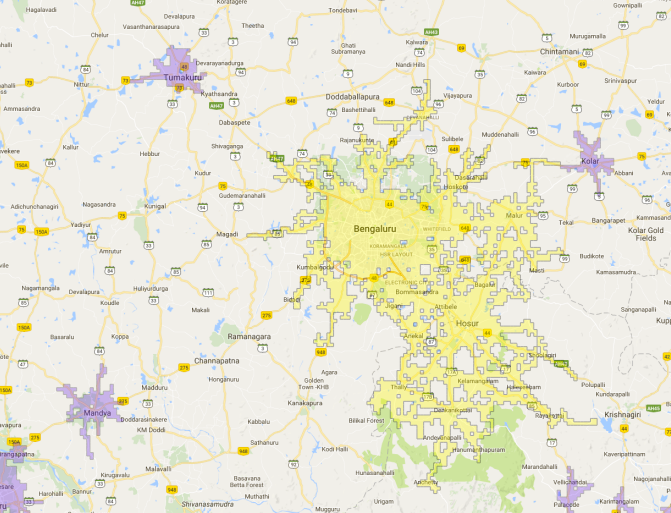
\includegraphics[width=\textwidth]{Bangalore}
  \caption{Geographic Definition of Bangalore}
   \label{fig:Bangalore}
\end{centering}
\end{figure}

\begin{table}
\caption{Regression Results}
\begin{center}
\begin{tabular}{lccc}
\multicolumn{4}{c}{\begin{large}Regional Mobility of Inventors and Productivity of Inventors\end{large}} \\ \hline
 & (1) & (2) & (3) \\
VARIABLES & Productivity & Productivity & Productivity \\ \hline
\vspace{4pt} & \begin{footnotesize}\end{footnotesize} & \begin{footnotesize}\end{footnotesize} & \begin{footnotesize}\end{footnotesize} \\
Moved Region (MR) & 1.5328*** & 0.8679*** & 0.5668*** \\
\vspace{4pt} & \begin{footnotesize}(0.2967)\end{footnotesize} & \begin{footnotesize}(0.1278)\end{footnotesize} & \begin{footnotesize}(0.0851)\end{footnotesize} \\
Prior Patents of Inventor (PPI) &  & 0.0866*** & 0.0740*** \\
\vspace{4pt} & \begin{footnotesize}\end{footnotesize} & \begin{footnotesize}(0.0065)\end{footnotesize} & \begin{footnotesize}(0.0019)\end{footnotesize} \\
Prior Patents of Team (PPT) &  & 0.0004* & 0.0005*** \\
\vspace{4pt} & \begin{footnotesize}\end{footnotesize} & \begin{footnotesize}(0.0002)\end{footnotesize} & \begin{footnotesize}(0.0002)\end{footnotesize} \\
MR x PPI &  &  & 0.0335*** \\
\vspace{4pt} & \begin{footnotesize}\end{footnotesize} & \begin{footnotesize}\end{footnotesize} & \begin{footnotesize}(0.0078)\end{footnotesize} \\
MR x PPT &  &  & -0.0006*** \\
\vspace{4pt} & \begin{footnotesize}\end{footnotesize} & \begin{footnotesize}\end{footnotesize} & \begin{footnotesize}(0.0002)\end{footnotesize} \\
Constant & 1.7242*** & 1.7335*** & 1.7487*** \\
 & \begin{footnotesize}(0.1644)\end{footnotesize} & \begin{footnotesize}(0.0746)\end{footnotesize} & \begin{footnotesize}(0.0848)\end{footnotesize} \\
\vspace{4pt} & \begin{footnotesize}\end{footnotesize} & \begin{footnotesize}\end{footnotesize} & \begin{footnotesize}\end{footnotesize} \\
Observations & 3,981,822 & 3,440,812 & 3,440,812 \\
$R^2$ & 0.0292 & 0.3001 & 0.3096 \\
Year FE & Yes & Yes & Yes \\
Technology FE & Yes & Yes & Yes \\
 Clustered SE & Country & Country & Country \\ \hline
\multicolumn{4}{c}{\begin{footnotesize} Robust standard errors in parentheses\end{footnotesize}} \\
\multicolumn{4}{c}{\begin{footnotesize} *** p$<$0.01, ** p$<$0.05, * p$<$0.1\end{footnotesize}} \\
\end{tabular}
\end{center}

\label{RC}
\end{table}

\begin{table}
\caption{Regression Results}
\begin{center}
\begin{tabular}{lccc}
\multicolumn{4}{c}{\begin{large}Country Mobility of Inventors and Productivity of Inventors\end{large}} \\ \hline
 & (1) & (2) & (3) \\
VARIABLES & Productivity & Productivity & Productivity \\ \hline
\vspace{4pt} & \begin{footnotesize}\end{footnotesize} & \begin{footnotesize}\end{footnotesize} & \begin{footnotesize}\end{footnotesize} \\
Moved Country (MC) & 1.8086*** & 0.9959*** & 0.6032*** \\
\vspace{4pt} & \begin{footnotesize}(0.1945)\end{footnotesize} & \begin{footnotesize}(0.0892)\end{footnotesize} & \begin{footnotesize}(0.1072)\end{footnotesize} \\
Prior Patents of Inventor (PPI) &  & 0.0860*** & 0.0774*** \\
\vspace{4pt} & \begin{footnotesize}\end{footnotesize} & \begin{footnotesize}(0.0041)\end{footnotesize} & \begin{footnotesize}(0.0036)\end{footnotesize} \\
Prior Patents of Team (PPT) &  & 0.0004*** & 0.0005*** \\
\vspace{4pt} & \begin{footnotesize}\end{footnotesize} & \begin{footnotesize}(0.0001)\end{footnotesize} & \begin{footnotesize}(0.0001)\end{footnotesize} \\
MC x PPI &  &  & 0.0332*** \\
\vspace{4pt} & \begin{footnotesize}\end{footnotesize} & \begin{footnotesize}\end{footnotesize} & \begin{footnotesize}(0.0083)\end{footnotesize} \\
MC x PPT &  &  & -0.0006 \\
\vspace{4pt} & \begin{footnotesize}\end{footnotesize} & \begin{footnotesize}\end{footnotesize} & \begin{footnotesize}(0.0006)\end{footnotesize} \\
Constant & 1.7019*** & 1.7212*** & 1.7294*** \\
 & \begin{footnotesize}(0.0871)\end{footnotesize} & \begin{footnotesize}(0.0453)\end{footnotesize} & \begin{footnotesize}(0.0483)\end{footnotesize} \\
\vspace{4pt} & \begin{footnotesize}\end{footnotesize} & \begin{footnotesize}\end{footnotesize} & \begin{footnotesize}\end{footnotesize} \\
Observations & 2,886,438 & 2,507,963 & 2,507,963 \\
$R^2$ & 0.0173 & 0.2903 & 0.2980 \\
Year FE & Yes & Yes & Yes \\
Technology FE & Yes & Yes & Yes \\
 Clustered SE & Region & Region & Region \\ \hline
\multicolumn{4}{c}{\begin{footnotesize} Robust standard errors in parentheses\end{footnotesize}} \\
\multicolumn{4}{c}{\begin{footnotesize} *** p$<$0.01, ** p$<$0.05, * p$<$0.1\end{footnotesize}} \\
\end{tabular}
\end{center}

\label{CR}
\end{table}

\end{document}

\begin{comment}
\begin{table}
\caption{Regression Results}
\begin{center}
\begin{tabular}{lccc}
\multicolumn{4}{c}{\begin{large}Mobility of Inventors and Productivity of Inventors\end{large}} \\ \hline
 & (1) & (2) & (3) \\
VARIABLES & Productivity & Productivity & Productivity \\ \hline
\vspace{4pt} & \begin{footnotesize}\end{footnotesize} & \begin{footnotesize}\end{footnotesize} & \begin{footnotesize}\end{footnotesize} \\
Moved Region (MR) & 1.0448*** & 0.4757*** & 0.5750*** \\
\vspace{4pt} & \begin{footnotesize}(0.0035)\end{footnotesize} & \begin{footnotesize}(0.0033)\end{footnotesize} & \begin{footnotesize}(0.0036)\end{footnotesize} \\
Moved Country (MC) & 0.9146*** & 0.6006*** & 0.0681*** \\
\vspace{4pt} & \begin{footnotesize}(0.0092)\end{footnotesize} & \begin{footnotesize}(0.0085)\end{footnotesize} & \begin{footnotesize}(0.0089)\end{footnotesize} \\
Prior Patents of Inventor (PPI) &  & 0.0785*** & 0.0716*** \\
\vspace{4pt} & \begin{footnotesize}\end{footnotesize} & \begin{footnotesize}(0.0001)\end{footnotesize} & \begin{footnotesize}(0.0001)\end{footnotesize} \\
Prior Patents of Team (PPT) &  & 0.0001*** & 0.0002*** \\
\vspace{4pt} & \begin{footnotesize}\end{footnotesize} & \begin{footnotesize}(0.0000)\end{footnotesize} & \begin{footnotesize}(0.0000)\end{footnotesize} \\
MR x PPI &  &  & -0.0053*** \\
\vspace{4pt} & \begin{footnotesize}\end{footnotesize} & \begin{footnotesize}\end{footnotesize} & \begin{footnotesize}(0.0002)\end{footnotesize} \\
MC x PPI &  &  & 0.0400*** \\
\vspace{4pt} & \begin{footnotesize}\end{footnotesize} & \begin{footnotesize}\end{footnotesize} & \begin{footnotesize}(0.0002)\end{footnotesize} \\
MR x PPT &  &  & 0.0002*** \\
\vspace{4pt} & \begin{footnotesize}\end{footnotesize} & \begin{footnotesize}\end{footnotesize} & \begin{footnotesize}(0.0000)\end{footnotesize} \\
MC x PPT &  &  & -0.0002*** \\
\vspace{4pt} & \begin{footnotesize}\end{footnotesize} & \begin{footnotesize}\end{footnotesize} & \begin{footnotesize}(0.0001)\end{footnotesize} \\
Constant & 1.5956*** & 1.3313*** & 1.3544*** \\
 & \begin{footnotesize}(0.0014)\end{footnotesize} & \begin{footnotesize}(0.0013)\end{footnotesize} & \begin{footnotesize}(0.0014)\end{footnotesize} \\
\vspace{4pt} & \begin{footnotesize}\end{footnotesize} & \begin{footnotesize}\end{footnotesize} & \begin{footnotesize}\end{footnotesize} \\
Observations & 4,368,107 & 3,721,250 & 3,721,250 \\
 $R^2$ & 0.0291 & 0.2721 & 0.2828 \\ \hline
\multicolumn{4}{c}{\begin{footnotesize} Standard errors in parentheses\end{footnotesize}} \\
\multicolumn{4}{c}{\begin{footnotesize} *** p$<$0.01, ** p$<$0.05, * p$<$0.1\end{footnotesize}} \\
\end{tabular}
\end{center}

\label{Ia}
\end{table}

\begin{frame}{Relevance of Answering the Research Question}{}
\begin{itemize}
\item{Received wisdom earlier was that firms would locate themselves in economic agglomerations to benefit from knowledge spillovers \citep{Jaffe1993}.}
\item{\cite{Zhao2006} has argued  that multinational enterprises may benefit from conducting R\&D in countries with weak IPR protection by  making up for the weaker IPR protection through better internal organization.}
\item{The anecdotal increase in the mobility of employees at the weak IPR subsidiaries raises a potential paradox.}
\item{If increased mobility of employees influences transfer of knowledge \citep{Almeida1999}, should we expect higher productivity  from inventors in those teams into which other inventors have moved in?}
\item{The answer to this question is not completely explained by theory}
\end{itemize}
\end{frame}

\begin{frame}{Managerial and Policy Implications}{}
\begin{itemize}
\item{The innovation policy of emerging countries is influenced with the expectation that the presence of multinational R\&D will create value adding spillover effects.}
\item{Productivity of innovation provides a richer proxy for value adding innovation, and effects of inventor mobility may inform innovation policy}
\item{Current work may inform managerial decisions about how to organize R\&D teams around the world}
\end{itemize}
\end{frame}


\cite{Zhao2006} argues that competing firms may have a lower ability to imitate when the value of technology is highly dependent on the proprietary firm\textquotesingle s internal resources. We contend that that assumption is weakened significantly if the knowledge of this technology is codified and published, and when published work on related technologies cite a common prior art. \cite{Zhao2006} herself cites \cite{Kogut1993} suggesting that difficult to codify knowledge lends itself to more efficient transfer within the firm. Drawing on \cite{Cohen2000}, we thereby conclude that firms would have a greater incentive to keep such highly dependent technology developed in weaker IPR countries secret, rather than make this knowledge public. While \cite{Zhao2006} highlights the strength of internal firm linkages in identifying and appropriating the knowledge generated in weak IPR location subsidiaries, she does not emphasize the importance of secrecy. Indeed, she uses patenting data from weaker IPR location offices to substantiate her hypothesis, which we believe actually weakens her argument for the strength of internal firm linkages.

\begin{longtable}{|p{0.5\textwidth}|p{0.30\textwidth}|}
\caption{Countries and their IPR scores \citep{Lesser2010}\label{long}}\\
 
 \hline\textbf{Country}&\textbf{IPR Score}\\\hline
 \endfirsthead
 
 \hline\textbf{Country}&\textbf{IPR Score}\\\hline
 \endhead
 
 \hline
 \endfoot
 
 \hline
 \endlastfoot
Afghanistan& \\\hline
Albania&4.7682 \\\hline
Algeria&2.7608 \\\hline
Angola&1.8734 \\\hline
Anguilla& \\\hline
Antigua and Barbuda& \\\hline
Argentina&5.4684 \\\hline
Armenia&4.4032 \\\hline
Aruba& \\\hline
Australia&11.1872 \\\hline
Austria&9.4024 \\\hline
Azerbaijan&3.1358 \\\hline
Bahamas& \\\hline
Bahrain&5.7736 \\\hline
Bangladesh&2.3664 \\\hline
Barbados& \\\hline
Belarus&3.2344 \\\hline
Belgium&9.6096 \\\hline
Belize& \\\hline
Benin& \\\hline
Bermuda& \\\hline
Bhutan&4.9300 \\\hline
Bolivia&4.2752 \\\hline
Bosnia and Herzegovina&2.9580 \\\hline
Botswana&6.2666 \\\hline
Brazil&5.2612 \\\hline
British Virgin Islands& \\\hline
Brunei Darussalam&5.4230 \\\hline
Bulgaria&5.3598 \\\hline
Burkina Faso&3.5496 \\\hline
Burma& \\\hline
Cambodia&1.9720 \\\hline
Cameroon&2.1692 \\\hline
Canada&11.1872 \\\hline
Cayman Islands& \\\hline
Central African Republic&1.9720 \\\hline
Chad&1.5776 \\\hline
Chile&9.2152 \\\hline
China&6.1586 \\\hline
Colombia&6.2572 \\\hline
Congo&1.8734 \\\hline
Cook Islands& \\\hline
Costa Rica&6.8388 \\\hline
Cote d'Ivoire&2.0706 \\\hline
Croatia&5.8528 \\\hline
Cuba& \\\hline
Cyprus&7.2526 \\\hline
Czech Republic&6.4444 \\\hline
Democratic Republic of the Congo&3.8260 \\\hline
Denmark&11.7788 \\\hline
Djibouti& \\\hline
Dominica& \\\hline
Dominican Republic& \\\hline
Ecuador&3.7822 \\\hline
Egypt&2.7608 \\\hline
El Salvador&3.3524 \\\hline
Equatorial Guinea& \\\hline
Estonia&9.1166 \\\hline
Ethiopia&2.6622 \\\hline
Fiji& \\\hline
Finland&11.3844 \\\hline
France&10.3984 \\\hline
French Guiana&10.3984 \\\hline
Gabon&2.8594 \\\hline
Gambia&2.8594 \\\hline
Georgia&4.9106 \\\hline
Germany&10.4970 \\\hline
Ghana&4.5904 \\\hline
Greece&5.4878 \\\hline
Greenland& \\\hline
Guadeloupe& \\\hline
Guam& \\\hline
Guatemala&3.3524 \\\hline
Guernsey& \\\hline
Guinea&1.7748 \\\hline
Guinea-Bissau& \\\hline
Guyana&2.5636 \\\hline
Haiti&1.7748 \\\hline
Honduras&3.2100 \\\hline
Hong Kong&8.0852 \\\hline
Hungary&7.6376 \\\hline
Iceland&10.1912 \\\hline
India&4.0974 \\\hline
Indonesia&4.5018 \\\hline
Iran (Islamic Republic of)&1.7748 \\\hline
Iraq&1.4790 \\\hline
Ireland&9.6290 \\\hline
Isle of Man& \\\hline
Israel&8.6236 \\\hline
Italy&6.8488 \\\hline
Jamaica&2.9580 \\\hline
Japan&10.2012 \\\hline
Jersey& \\\hline
Jordan&6.5430 \\\hline
Kazakhstan&2.6622 \\\hline
Kenya&3.7822 \\\hline
Korea, Democratic Republic of& \\\hline
Korea, Republic of&7.1640 \\\hline
Kuwait&4.0426 \\\hline
Kyrgyzstan&3.4864 \\\hline
Lao People's Democratic Republic&1.9720 \\\hline
Latvia&6.0500 \\\hline
Lebanon&2.4650 \\\hline
Lesotho& \\\hline
Liberia&3.0566 \\\hline
Libyan Arab Jamahiriya& \\\hline
Liechtenstein& \\\hline
Lithuania&7.4404 \\\hline
Luxembourg&8.8302 \\\hline
Macau& \\\hline
Madagascar&2.9580 \\\hline
Malawi&3.2538 \\\hline
Malaysia&5.1820 \\\hline
Mali&2.7608 \\\hline
Malta& \\\hline
Mauritania&2.4650 \\\hline
Mauritius&5.3244 \\\hline
Mexico&4.8668 \\\hline
Monaco& \\\hline
Mongolia&3.4072 \\\hline
Montenegro& \\\hline
Morocco&5.8628 \\\hline
Mozambique&2.4650 \\\hline
Namibia&4.4370 \\\hline
Nepal&2.2678 \\\hline
Netherlands Antilles&11.3844 \\\hline
Netherlands&11.3844 \\\hline
New Caledonia& \\\hline
New Zealand&11.8774 \\\hline
Nicaragua&5.0740 \\\hline
Niger&2.8594 \\\hline
Nigeria&3.2100 \\\hline
Northern Mariana Islands& \\\hline
Norway&10.1912 \\\hline
Oman&7.0360 \\\hline
Pakistan&4.1074 \\\hline
Palau& \\\hline
Palestine& \\\hline
Panama&5.2164 \\\hline
Papua New Guinea&2.0706 \\\hline
Paraguay&3.6836 \\\hline
Peru&5.3892 \\\hline
Philippines&4.1074 \\\hline
Poland&7.5390 \\\hline
Portugal&8.3278 \\\hline
Puerto Rico& \\\hline
Qatar&7.6470 \\\hline
Republic of Moldova&4.1218 \\\hline
Reunion& \\\hline
Romania&6.3558 \\\hline
Russia&4.0332 \\\hline
Saint Barthelemy& \\\hline
Saint Kitts and Nevis& \\\hline
Saint Lucia& \\\hline
Saint Pierre and Miquelon& \\\hline
San Marino& \\\hline
Saudi Arabia&4.2398 \\\hline
Senegal&2.9580 \\\hline
Serbia&4.4470 \\\hline
Seychelles& \\\hline
Sierra Leone&2.1692 \\\hline
Singapore&11.6802 \\\hline
Slovakia&7.0460 \\\hline
Slovenia&8.3716 \\\hline
Solomon Islands& \\\hline
South Africa&7.2432 \\\hline
Spain&8.6236 \\\hline
Sri Lanka&3.0566 \\\hline
Sudan&1.4790 \\\hline
Suriname&3.6482 \\\hline
Svalbard& \\\hline
Swaziland&4.2946 \\\hline
Sweden&11.6802 \\\hline
Switzerland&11.4830 \\\hline
Syrian Arab Republic&3.5596 \\\hline
Taiwan&7.2626 \\\hline
Tajikistan&1.9720 \\\hline
Thailand&4.0974 \\\hline
The former Yugoslav Republic of Macedonia& \\\hline
Togo&2.7608 \\\hline
Trinidad and Tobago&5.1626 \\\hline
Tunisia&5.8528 \\\hline
Turkey&6.9474 \\\hline
Turkmenistan& \\\hline
Turks and Caicos Islands& \\\hline
Uganda&2.4650 \\\hline
Ukraine&3.7822 \\\hline
United Arab Emirates&6.4090 \\\hline
United Kingdom&10.2012 \\\hline
United Republic of Tanzania&2.5636 \\\hline
United States Virgin Islands&10.0040 \\\hline
United States&10.0040 \\\hline
Uruguay&8.2192 \\\hline
Uzbekistan&3.6388 \\\hline
Venezuela&3.6144 \\\hline
Vietnam&4.2752 \\\hline
Yemen&2.0706 \\\hline
Zambia&2.9580 \\\hline
Zimbabwe&2.9142 \\\hline
\end{longtable}



\end{comment}
